\chapter{Results and Evaluation}

This chapter presents the results and findings from this work in extracting bounded contexts within FTAPI's software ecosystem. Building upon the five-phase workflow established in Chapter 6, we analyze how Large Language Models performed across each stage of the Domain Driven Design process. From establishing a ubiquitous language to proposing technical architecture mappings. The results reveal both the cpapbilities and limitations of current AI models in supporting domain modeling efforts.

\section{Capturing Ubiquitous Language}
The LLM's were first tasked to capture the ubiquitous language from a large requirements set. This initial phase formed the foundation for the whole subsequent architecural analysis, as establishing a consistent domain vocabulary is fundamental to the domain driven design process. The models were provided with requirement sets for both Securoom and Secumail domains from FTAPI's product marketing material

\subsection{Securooms}
The SecuRooms requirements, produced remarkably consistent core vocabulary across all three models. The Table \ref{tab:securooms-ubiquitous-language} presents a comparative analysis of key domain terms extracted by each LLM. All models successfully identified the central concept of a "SecuRoom" as a secure container for file collaboration, though their specific definitions revealed subtle differences in understanding. Claude emphasized the optional nature of end-to-end encryption, reflecting the product's flexibility, while Gemini focused on the SecuRoom as the primary workspace and access boundary. GPT provided the most architecturally-oriented definition, explicitly mentioning "security and access boundary" as defining characteristics. Particularly noteworthy was the treatment of "SecuPass," the personal password protecting users' private keys for end-to-end encryption. All models correctly identified its critical security function and irrecoverable nature. Claude and Gemini explicitly noted that without the SecuPass, encrypted content becomes permanently inaccessible—a crucial business invariant that GPT captured more implicitly through the term "personal credential."

\begin{table}[H]
    \centering
    \begin{tabular}{|p{2.5cm}|p{4cm}|p{4cm}|p{4cm}|}
    \hline
    \rowcolor{gray!20}
    \textbf{Term} & \textbf{Claude Opus 4.1} & \textbf{Gemini 2.5 Pro} & \textbf{GPT 5.0} \\
    \hline
    \textbf{SecuRoom} & 
    Secure virtual container for storing, sharing, and collaborating on files, with optional E2E encryption. &
    Secure virtual container for files/folders, primary workspace and access boundary. &
    Protected digital workspace grouping files, folders, and participants under a defined security and access boundary. \\
    \hline
    \textbf{Owner} & 
    Member with full control, including deletion and member management. &
    Role with total control: manage members, change roles, delete the room. &
    Primary authority: governs lifecycle, invites/removes members, assigns roles, deletes SecuRoom. \\
    \hline
    \textbf{Member} & 
    User who accepted an invitation and has an active role. &
    User granted access and assigned a role; becomes member of a room. &
    Participant with access rights and defined role; scoped to one SecuRoom. \\
    \hline
    \textbf{Pending Member} & 
    Invited user who has not yet completed signup/acceptance. &
    Temporary status: registered via invitation but awaiting final approval. &
    User invited but not yet active until confirmation/approval. \\
    \hline
    \textbf{SecuPass} & 
    Personal, irrecoverable password protecting user's private key for E2E encryption. &
    User-specific password unlocking private key for E2E decryption. &
    Personal credential unlocking private key; without it, user cannot decrypt/access content. \\
    \hline
    \rowcolor{gray!10}
    \textit{Other Terms} & 
    25+ additional (e.g., Invitation, Folder Permission, Re-encryption, Audit Trail). &
    ~15 additional (e.g., Role, Invitation, Access Grant, File, Audit Trail). &
    ~15 additional (e.g., Role, Invitation, Access Grant, File, Folder, Annotation, Retention Policy). \\
    \hline
    \end{tabular}
    \caption{Comparison of domain terms for Securooms across Claude Opus 4.1, Gemini 2.5 Pro, and GPT 5.0.}
    \label{tab:securooms-ubiquitous-language}
\end{table}


\subsection{Secumails}

The SecuMails requirements produced consistent vocabulary extraction across the three models, though with notable variations reflecting the domain's monolithic complexity and accumulated technical debt. Table \ref{tab:secumails-ubiquitous-language} presents a comparative analysis of key domain terms extracted by each LLM. All models successfully identified "Delivery" as the core concept for secure message transfer. Claude emphasized its immutable nature—"once sent, cannot be modified"—capturing a fundamental business constraint. Gemini provided a structural definition highlighting the delivery as "the core container for a secure transfer" with subject, message, and attachments. GPT framed it as a "secure unit" emphasizing both security and flexibility in recipient handling. The "SubmitBox" concept demonstrated consistent understanding across models as a secure digital mailbox for external submissions, though with varying emphasis. Claude focused on ownership ("owned by a user"), Gemini stressed uniqueness and security per user, while GPT noted broader applicability to both users and organizations.

\begin{table}[H]
    \centering
    \begin{tabular}{|p{2.5cm}|p{4cm}|p{4cm}|p{4cm}|}
    \hline
    \rowcolor{gray!20}
    \textbf{Term} & \textbf{Claude Opus 4.1} & \textbf{Gemini 2.5 Pro} & \textbf{GPT 5.0} \\
    \hline
    \textbf{Delivery} & 
    An immutable package containing message and/or attachments that, once sent, cannot be modified &
    The core container for a secure transfer. It consists of a subject, a message, and zero or more Attachments, which is sent to one or more Recipients. &
    A secure unit containing a subject, a message, and optional file attachments. A delivery can be sent to one or multiple recipients \\
    \hline
    \textbf{Submitbox} & 
    Personal digital mailbox owned by a user for receiving external submissions&
    A personal, secure "digital mailbox," unique to each User, that allows external parties to send them files. &
    A secure digital mailbox that allows external parties to upload files/messages to an FTAPI user or organization. \\
    \hline
    \textbf{Recipient} & 
    Person who receives an Access Grant to a Delivery &
    The intended actor who receives a Delivery. Can be an internal User or an external party. &
    A person who receives a delivery. Can be either a Registered Recipient (User) with a full FTAPI account or a Guest Recipient created automatically at Security Level 2+, with restricted access. \\
    \hline
    \rowcolor{gray!10}
    \textit{Other Terms} & 
    ~35 additional (e.g., Secupass, Role, License, ...). &
    ~40 additional (e.g., Sender, Secupass, Notification, ...). &
    ~35 additional (e.g., Role, Secupas, Security Level, ...). \\
    \hline
    \end{tabular}
    \caption{Comparison of domain terms for Secumails across Claude Opus 4.1, Gemini 2.5 Pro, and GPT 5.0.}
    \label{tab:secumails-ubiquitous-language}
\end{table}

\section{Event Storming}
The second phase of the analysis focused on simulating event storming sessions with the Large Language Models to identify event flows and behaviors within each domain. Building upon the established ubiquitous language, the LLMs were tasked with mapping out and identifying domain events. The second phase of the analysis focused on simulating event storming sessions with the Large Language Models to identify event flows and behaviors within each domain. Building upon the established ubiquitous language, the LLMs were tasked with mapping out and identifying domain events. This exercise revealed how different models interpret temporal sequences and business processes, with varying levels of technical detail and abstraction that significantly influenced the resulting architectural proposals.

\subsection{Securooms}
The event storming simulation for SecuRooms produced similar event flows across all three models, with particular consistency in identifying core workflows. The activity diagram in Figure \ref{fig:event-create-securoom-claude} shows an example for the creation process of a SecuRoom. The LLM correctly identified that there are rules for creating the SecuRoom and also that there are potential encryption requirements depending on if the room is end-to-end encrypted.

\begin{figure}[H]
    \centering
    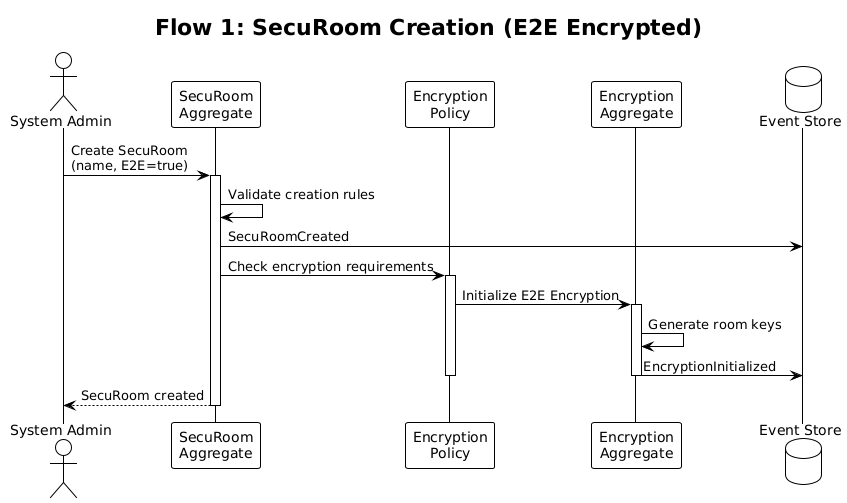
\includegraphics[height=5cm]{figures/create-securoom-claude.png} 
    \caption{Create Securoom Claude 4.1 Opus}
    \label{fig:event-create-securoom-claude} 
  \end{figure}

Figure \ref{fig:event-create-securoom-claude} identified by Gemini shows an example of a more complex event flow: inviting a new user to an end-to-end encrypted SecuRoom. Because of the complexity of the process, this is a multi-step procedure. What is particularly notable here is that the LLM already tries to identify aggregate and the responsabilities of those aggregates.

\begin{figure}[H]
    \centering
    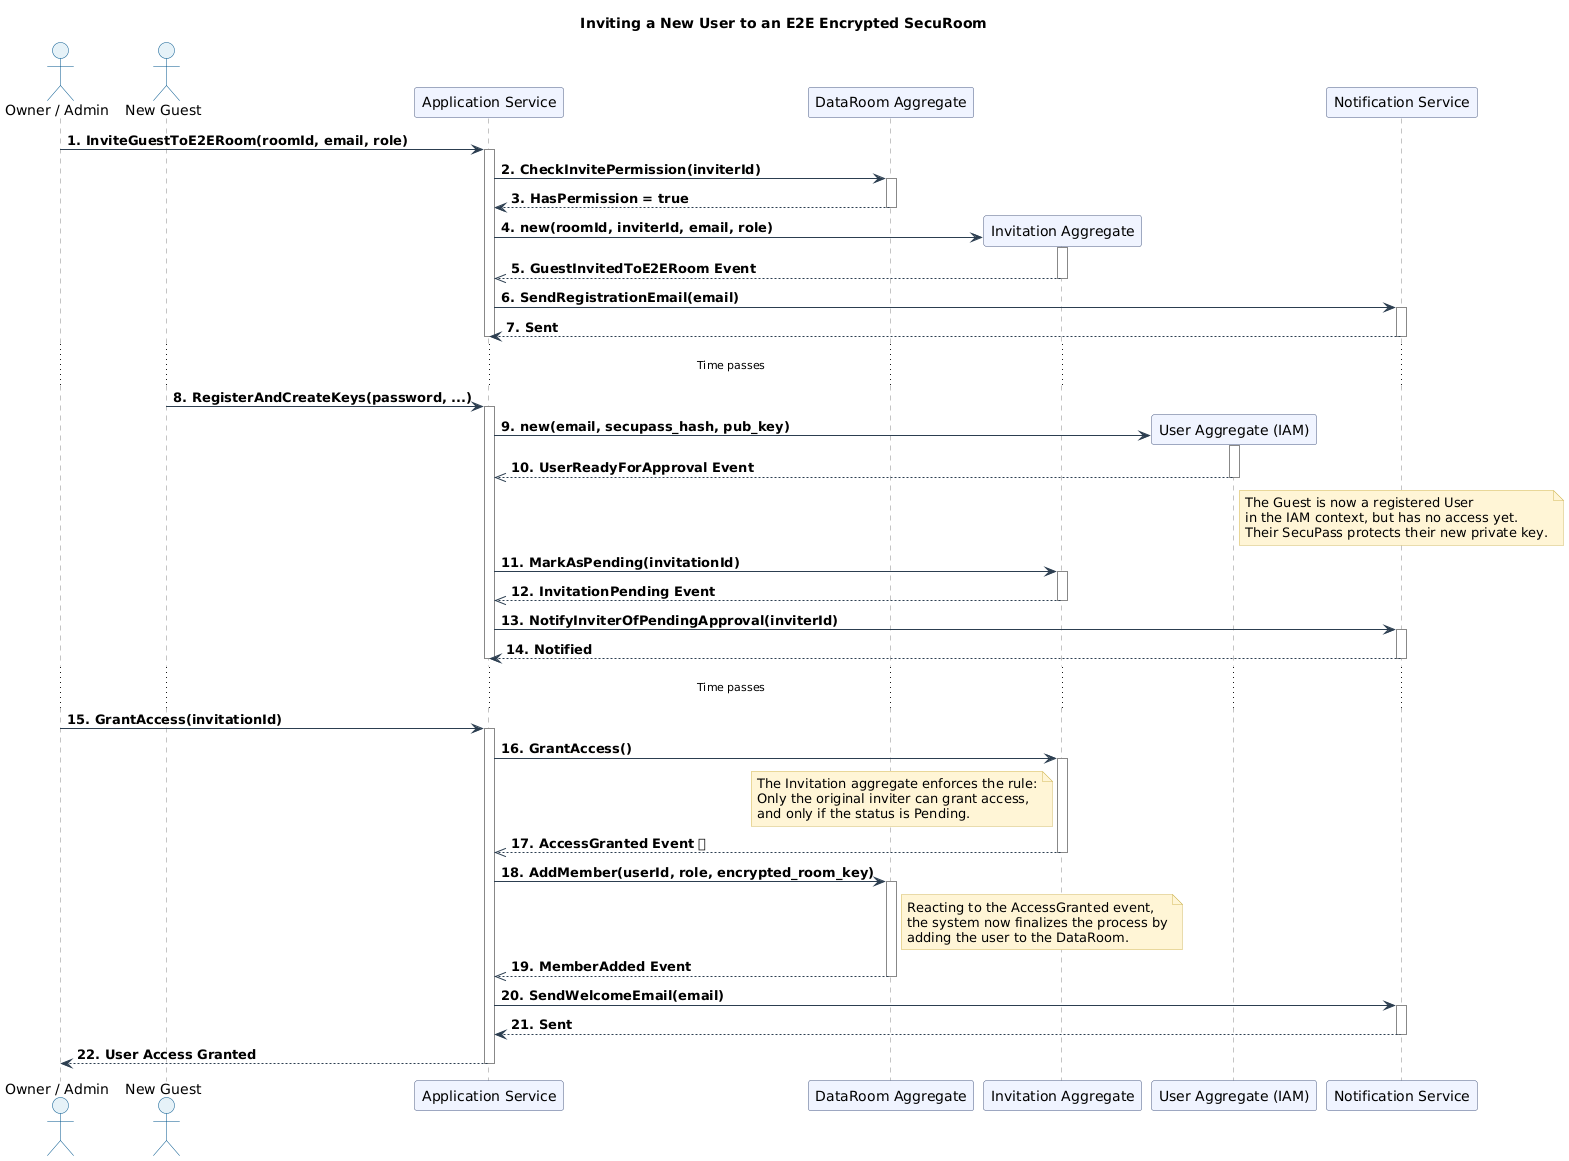
\includegraphics[height=7cm]{figures/invitaion-new-user-gemini.png} 
    \caption{Invitation of a new user to a Securoom - Gemini 2.5 Pro}
    \label{fig:event-invite-new-user-gemini} 
  \end{figure}

  \subsection{SecuMails}

  For SecuMails we performed the same event storming steps, but with the larger requirements set the LLMs seemed to struggle with displaying it in a similar manner as in the SecuRooms domain. The years of accumulated features meant there were simply many more events to identify and connect.
  
  Claude took an interesting approach to handle this complexity. Figure \ref{fig:event-stormin-secumails-1} shows the first step where Claude wrote out all events in a list format, basically creating an inventory of everything that happens in the SecuMails domain. This list ended up with over 45 different events covering everything from delivery creation to encryption to notifications.
  
  \begin{figure}[htbp]
    \centering
    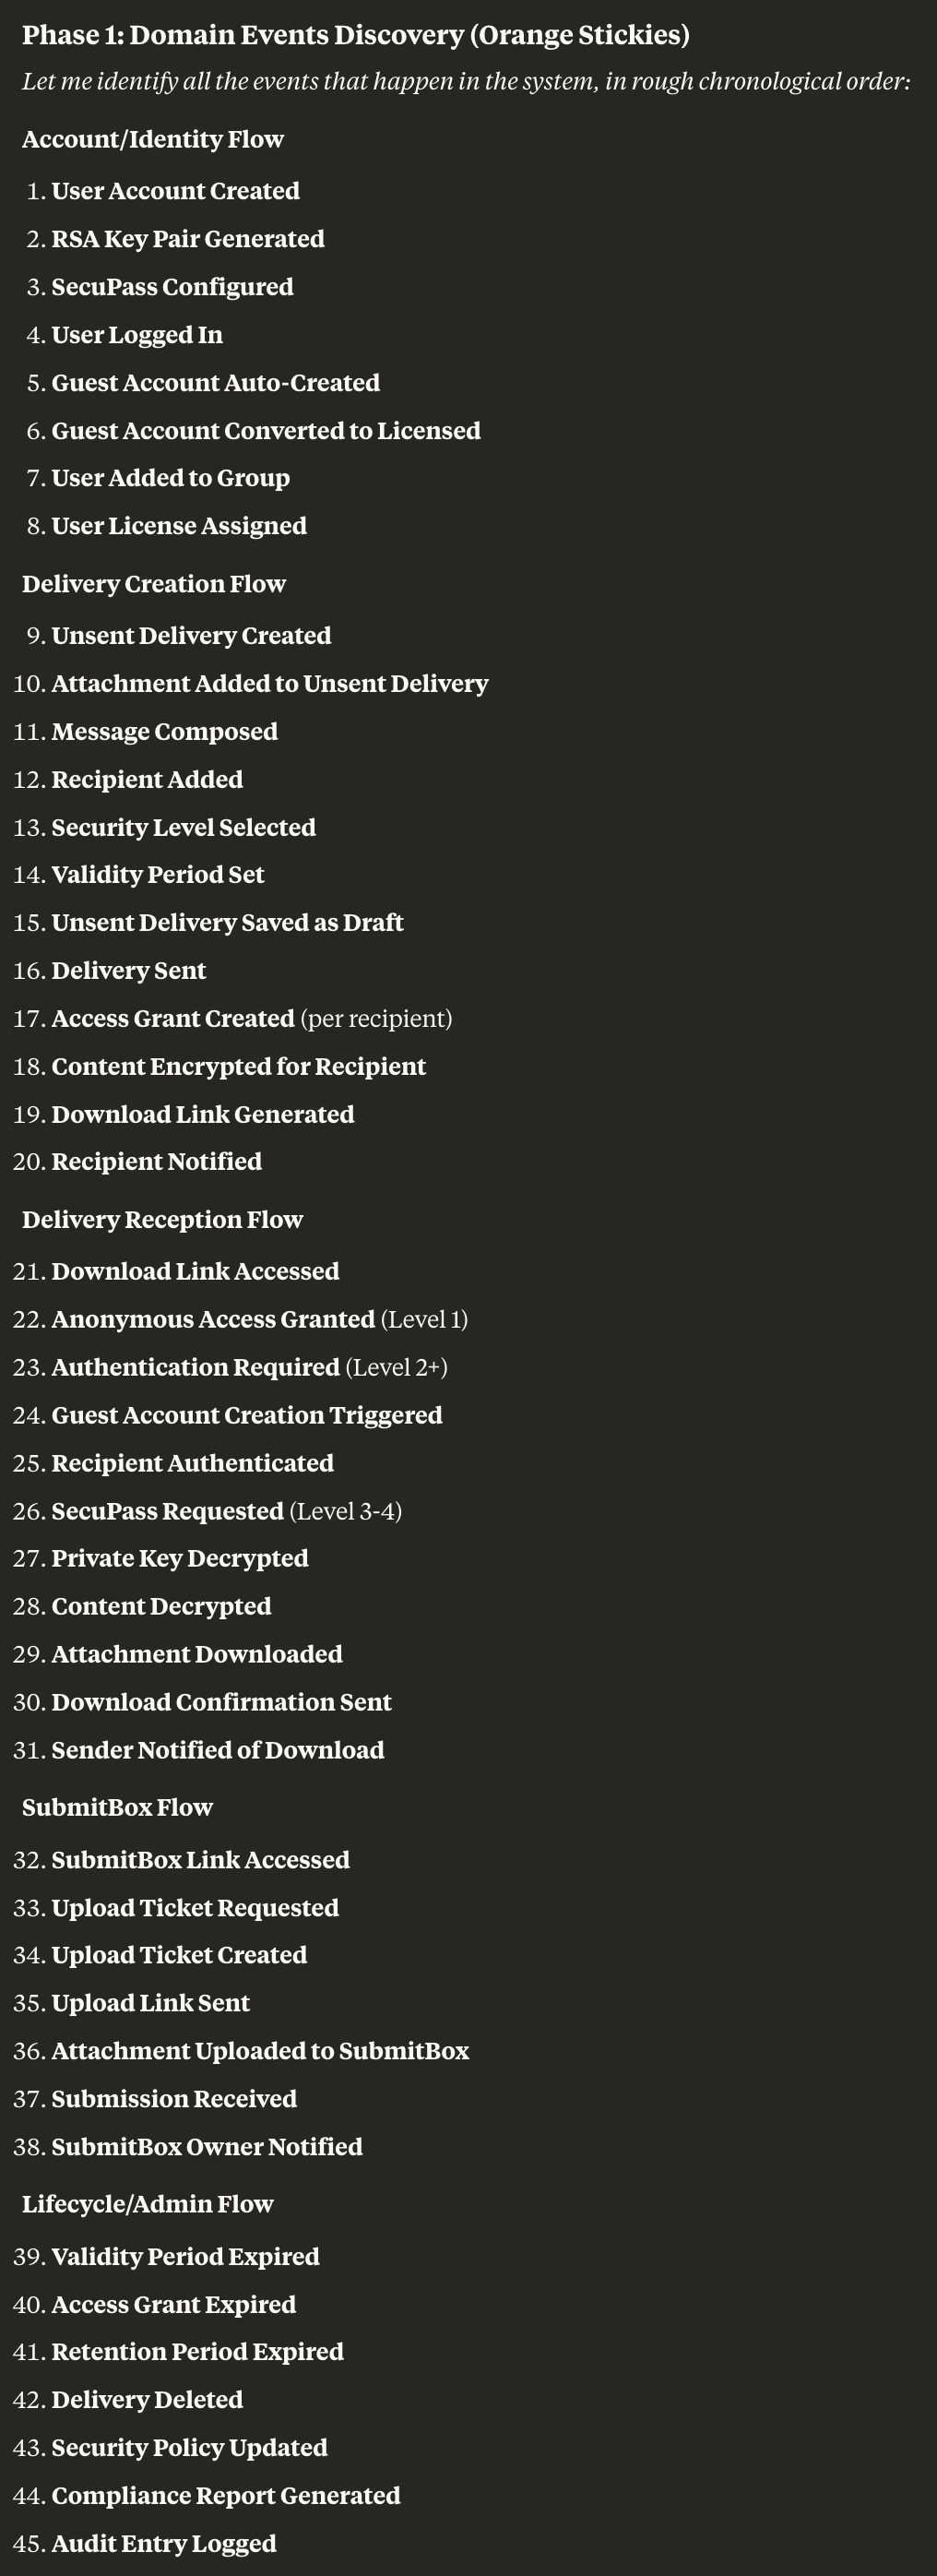
\includegraphics[height=7cm]{figures/secumails-event-storming-claude-1.png} 
    \caption{Event list extraction for SecuMails - Claude 4.1 Opus}
    \label{fig:event-stormin-secumails-1} 
  \end{figure}
  
  As seen in Figure \ref{fig:event-stormin-secumails-2}, Claude then tried to combine these individual events into actual flows. This helped make sense of the complexity and was more readable than when trying to prompt Claude to display the events in a diagram like in the SecuRooms domain. The model grouped related events together, identifying patterns like the delivery lifecycle and encryption workflows, though the connections between different flows remained complex.
  
  \begin{figure}[htbp]
    \centering
    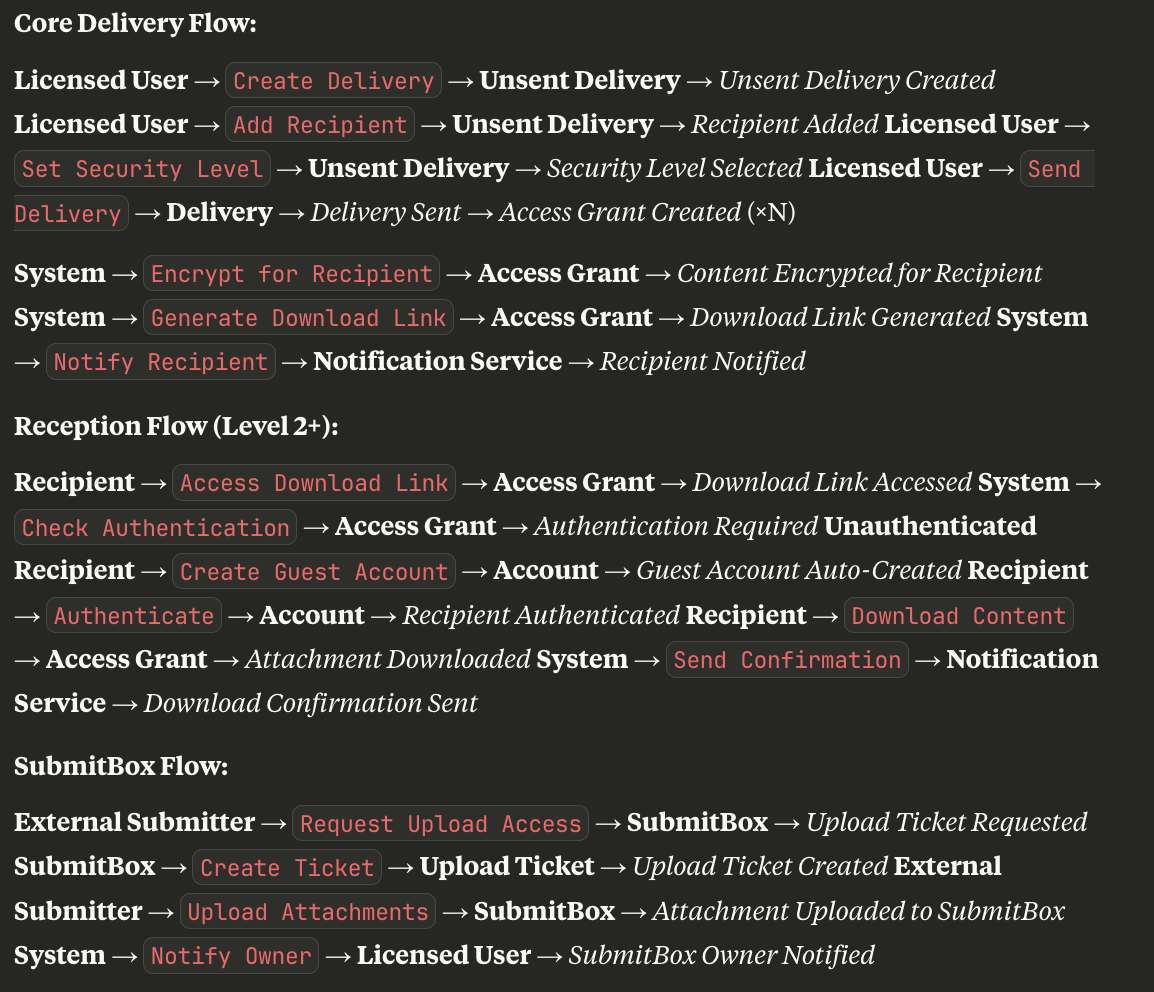
\includegraphics[height=7cm]{figures/secumails-claude-event-storming-2.png} 
    \caption{Event flow organization for SecuMails - Claude 4.1 Opus}
    \label{fig:event-stormin-secumails-2} 
  \end{figure}
  
  Figure \ref{fig:diagram-event-storming-claude-1} shows what happened when we asked Claude to create a visual diagram similar to the SecuRooms ones. The diagram became extremely complex due to the sheer number of events that Claude tried to display at once. This visualization challenge really highlights the difference between the clean SecuRooms architecture and the entangled SecuMails monolith—where SecuRooms events follow clear paths, SecuMails events branch and interconnect in ways that are difficult to represent visually.
  
  \begin{figure}[htbp]
    \centering
    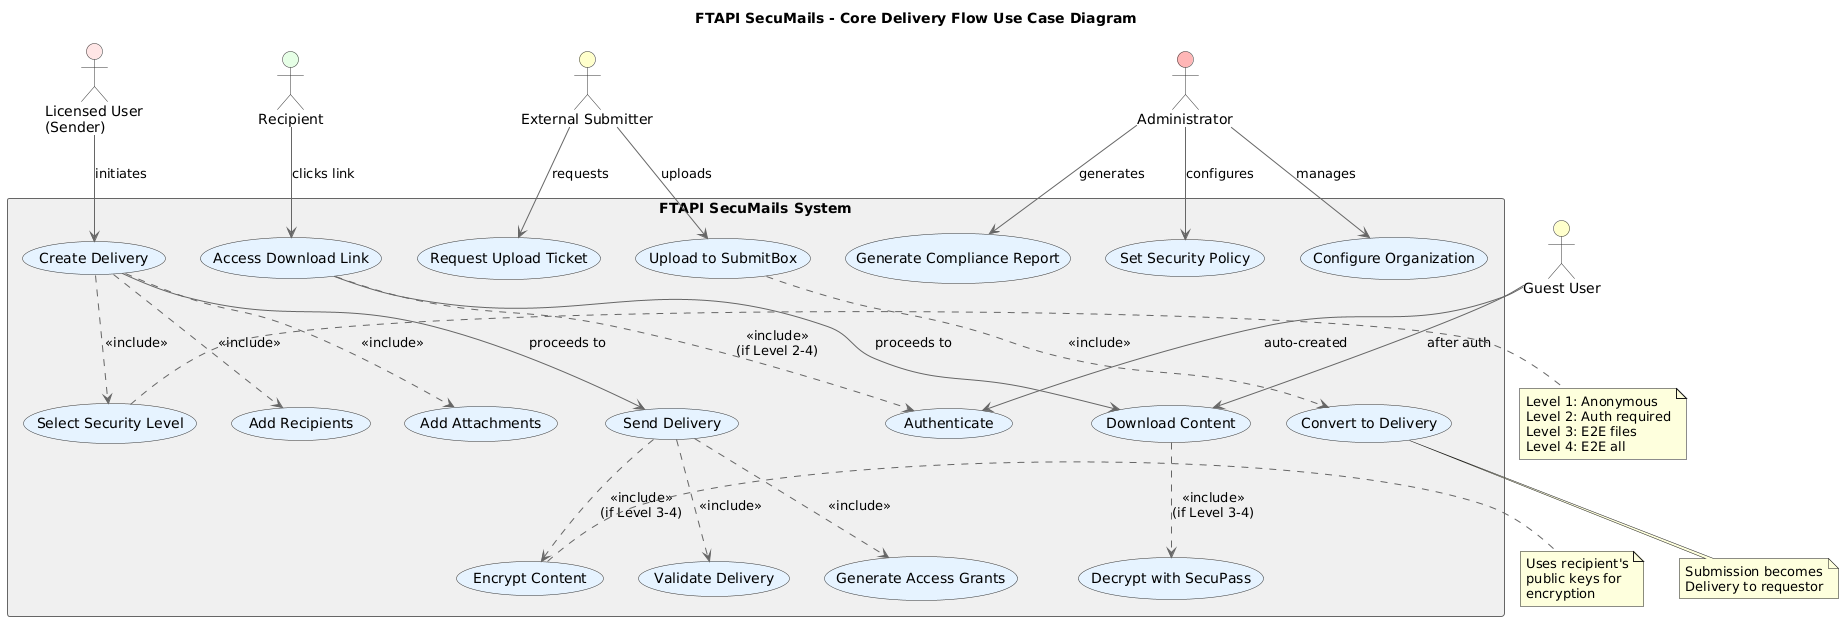
\includegraphics[height=5cm]{figures/diagram-secumail-event-1.png} 
    \caption{Complex event diagram attempt for SecuMails - Claude 4.1 Opus}
    \label{fig:diagram-event-storming-claude-1} 
  \end{figure}

\section{Proposed Bounded Contexts}

\subsection{Securooms}
\begin{figure}[htbp]
  \centering
  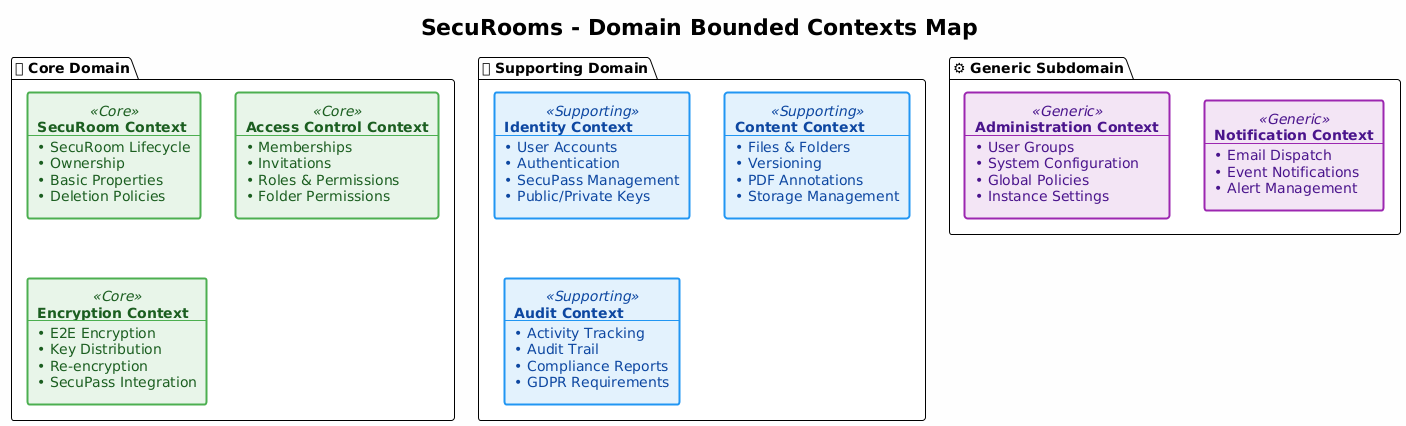
\includegraphics[height=5cm]{figures/bounded-context-securoom-claude.png} 
  \caption{Secumails proposed Bounded Contexts - Claude 4.1 Opus}
  \label{fig:diagram-bounded-contexts-secumail-claude} 
\end{figure}

\subsection{Secumails}
insert images and descriptions of proposals

\section{Aggregates}

show examples of proposed aggregates

\section{Architecture Mapping}

show examples of proposed architecture mappings

\section{Expert Evaluation Results}

\subsection{SecurRooms: Comparison Against a Known Benchmark}

Experts were in general agreement that the LLM-extracted ubiquitous language was 'surprisingly accurate' for core concepts, providing definitions that were both robust and closely aligned with current internal terminology. Expert A noted that the clarifying questions posed by the LLM closely mirrored the discovery process the human team experienced when initially defining these terms. For instance, the LLM correctly identified the synonymous use of 'SecuRoom' and 'Dataroom' within the requirements and prompted for a single, authoritative business term, demonstrating its ability to resolve linguistic ambiguity.

\subsection{Securroms}

\subsection{Secumails}

\subsection{Overall impression and conclusion}